\documentclass[a4paper]{article}

\usepackage[]{babel}
\usepackage[latin1]{inputenc}
\usepackage{amssymb}
\usepackage{framed}
\setlength{\parindent}{0pt}
\setlength{\parskip}{3ex}
\usepackage{tikz}
\usepackage{biblatex}
\usepackage{graphicx} % Required for including images
\usepackage{subcaption} % Required for creating subfigures


\bibliography{Labs/Lab 4/ref}

\begin{document}

\begin{center}
  {\large Artificial Neural Networks and Deep Architectures, DD2437}\\
  \vspace{7mm}
  {\huge Short report on lab assignment 4\\[1ex]}
  {\Large Restricted Boltzmann Machines and
Deep Belief Nets}\\
  \vspace{8mm}  
  {\Large Rakin Ali, Steinar Logi and Hassan Alzubeidi\\}
  \vspace{4mm}
  {\large March 4, 2024\\}
\end{center}



\section{Main objectives and scope of the assignment}

The main objective with this lab is to familiarize ourselves with Deep Belief Nets (DBN). Deep belief nets are a Deep Neural Network architecture combined of multiple Restricted Boltzmann Machines that are pre-trained using unsupervised greedy pre-training, using Contrastive Divergence. The main objectives are the following:  
\begin{itemize}
\item To Familiarize ourselves with the key ideas underlying the learning process of Restricted Boltzmann Machines.
\item Design a Deep Belief Network and train it using greedy pre-training.
\item Study the Generative aspects of DBN
\end{itemize}
Deep Neural Network architectures are a class of many different networks that can exploit the expressive powers of deep architectures, for example using Autoencoders to pre-train the hidden layers. In this lab we will, however, focus on a certain subset of deep architectures, namely Deep Belief Nets, which use Restricted Boltzmann Machines.

\section{Methods}
A code skeleton was generated for us to use however all of us modified it to be able to complete this lab. All of us did this separately which gave us better insights on how to build the models however only one of us could complete the lab code-wise fully. 

\section{Results and discussion}
Section \ref{part1} covers task 4.1 where an RBM was used for recognizing MNIST images. Section \ref{part2} covers greedy layer-wise pertaining which corresponds to section 4.2. Most of the ideas were taken from the two reports by Hinton \cite{hinton2006fast} \cite{hinton2012practical}. The one which came out recently was more useful for this lab. 

\subsection{Restricted Bolzmann Machine}
\label{part1}
Restricted Boltzmann Machines (RBMs) have hidden nodes and visible nodes. The activations of the nodes are probabilistic and not deterministic. Each node is a sigmoid activation function and the input is the weighted sum of all the other nodes. The activation is the probability of node being turned on or not. The mathematical notation for it can be seen below:
$$
p(v_i = 1) = \sigma (\sum_i w_{ij}v_{i})
$$
The Restricted Boltzmann machine is a subset of Boltzmann Machines where connections within layers are omitted. The Restricted Boltzmann Machine can therefore be represented as bipartide graph. When there are no connections within the layer, the visible nodes are conditionally independent given the hidden nodes and vice versa, that is:
$$
p(\textbf{v} |  \textbf{h}) = \Pi_{i}p(v_i | \textbf{h})
$$
The Restricted Boltzmann Machine is trained using Contrastive Divergence. To use Contrastive Divergence we need to perform alternating Gibbs sampling on the network to obtain the updates of the weights. The update between the ith visible unit and jth hidden unit is: $\Delta w_{ij} \propto <v_i h_j>^{t=0} - <v_i h_j>^{t=k}$. What Contrastive Divergence essentially does is that it maximizes the likelihood of the joint probability $p(\textbf{v}, \textbf{h})$. That is the visible states in the dataset are assigned maximum probability. The hidden vectors therefore describe some latent features of the data set that we assume are useful. This is then exploited in Deep Belief Networks by pre-training separate Restricted Boltzmann Machines. We will see this in part 2 of this lab.

Monitoring stability was an interesting task, According to the literature, \textit{"the construction error is actually a very poor measure of the progress of learning"} \cite{hinton2012practical}. In short terms use it but don't trust it. If you want to know if it is learning then use graphic displays and analyze the weights and see what they have learned. This was done and can be seen in figure \ref{fig:Lab4-comparison}. 
\begin{figure}[htb]
    \centering
    \begin{subfigure}[b]{0.45\textwidth}
        \centering
        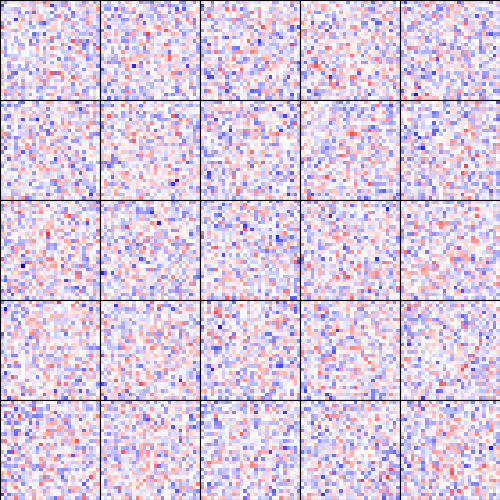
\includegraphics[width=\textwidth]{Labs/Lab 4/Steinar/rf.iter000000.png}
        \caption{No iterations}
        \label{fig:Lab4-iter1}
    \end{subfigure}
    %
    \begin{subfigure}[b]{0.45\textwidth}
        \centering
        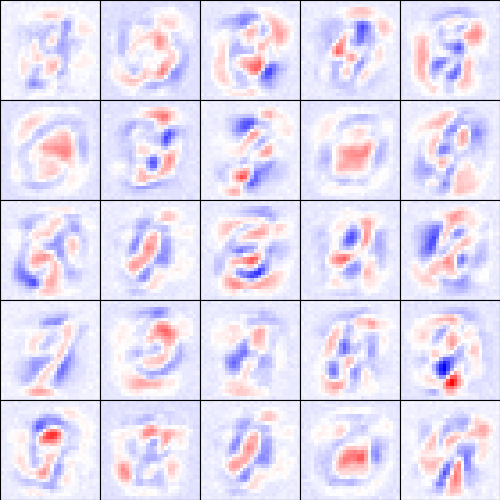
\includegraphics[width=\textwidth]{Labs/Lab 4/Steinar/rf.iter000001.png}
        \caption{First Iteration of Contrastive Divergence}
        \label{fig:Lab4-iter2}
    \end{subfigure}
    \caption{Comparison of Contrastive Divergence iterations}
    \label{fig:Lab4-comparison}
\end{figure}

We created a Restricted Boltzmann Machine and trained it using Contrastive Divergence. We used the MNIST dataset with handwritten digits. Each image in this data set is 28 by 28 pixels, that is each input vector when flattened has 784 dimensions. We split the dataset into a training set and test set. We used a Restricted Boltzmann Machine with 500 hidden units and trained it using Contrastive Divergence on the training set. We used a batch size of 20 and trained the Restricted Boltzmann Machine for 30 epochs. By tracking the reconstruction error we noticed that we could monitor if the RBM achieved some kind of stability. The reconstruction error was calculated by clamping the input to the visible nodes and the calculating the probabilities of the hidden nodes given the input and then calculating the probabilities of the visible nodes given the hidden probabilities. We then measured the distance of the reconstructions from the original images using np.linalg.norm function in numpy. We plotted the reconstruction loss as a function of epoch and the results from that can be seen in figure \ref{fig:reconstruction-convergence}. As can be seen in the figure some kind of convergence seems to be achieved. The reconstruction error seems to stabilize after a few iterations.

\begin{figure}[ht]
    \centering
    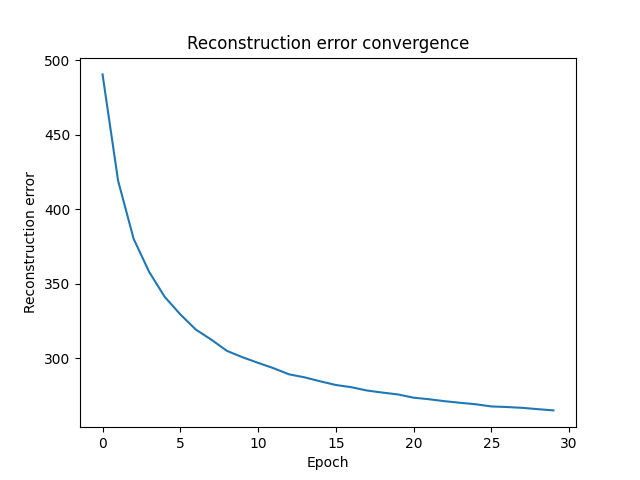
\includegraphics[width=0.5\textwidth]{Labs/Lab 4/Steinar/reconstruction_convergence.png}
    \caption{Convergence of the reconstruction error}
    \label{fig:reconstruction-convergence}
\end{figure}
Below are images of how the total amount of hidden node affects reconstruction loss:

\begin{figure}[htb]
    \centering
    \begin{subfigure}[b]{0.45\textwidth}
        \centering
        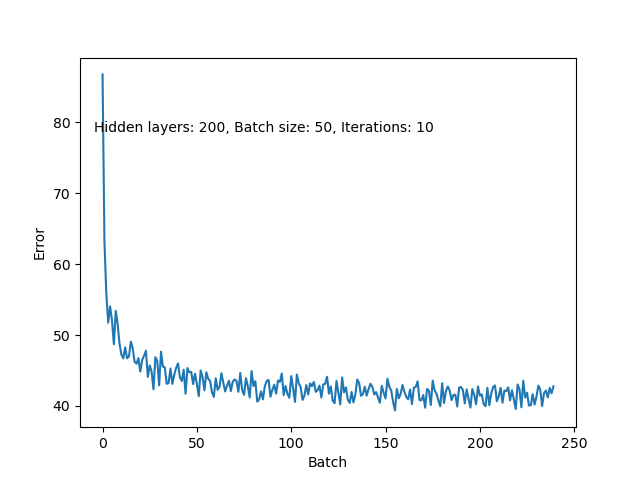
\includegraphics[width=\textwidth]{Labs/Lab 4/Rakin/plots/Hidden_layers_200_batch_50_iterations_10.png}
        \caption{No iterations}
        \label{fig:Lab4-iter1}
    \end{subfigure}
    %
    \begin{subfigure}[b]{0.45\textwidth}
        \centering
        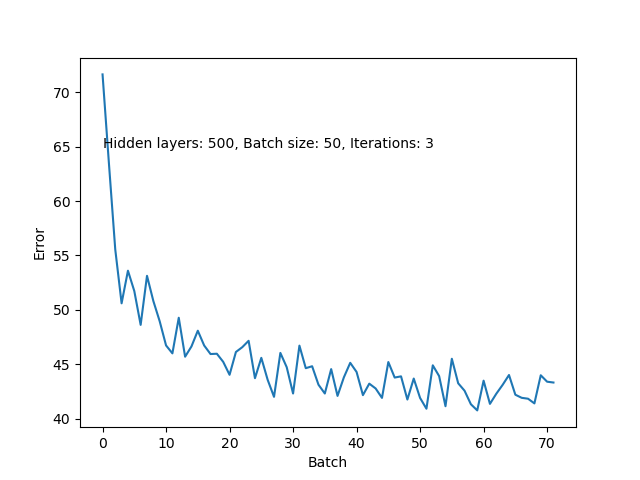
\includegraphics[width=\textwidth]{Labs/Lab 4/Rakin/plots/Hidden_layers_500_batch_50_iterations_3.png}
        \caption{First Iteration of Contrastive Divergence}
        \label{fig:Lab4-iter2}
    \end{subfigure}
    \caption{Comparison of None and First Iteration}
    \label{fig:Lab4-comparison-hiddenNodes}
\end{figure}

\subsection{Greedy-later-wise Pretraining}
\label{part2}
In part one we pre-trained a single RBM using contrastive divergence. In this part the RBMs class which we completed from task 1 was imported and used to Stack the RBMs. The different RBMs and how they were stacked in order to create a Deep Belief network (DBN) can be bee seen below in figure \ref{fig:rbm_stack}. Bear in mind all except labels are RBMs which are pre-trained. Each RBM extracts a representation of the data. 

\begin{figure}[htb]
  \centering
  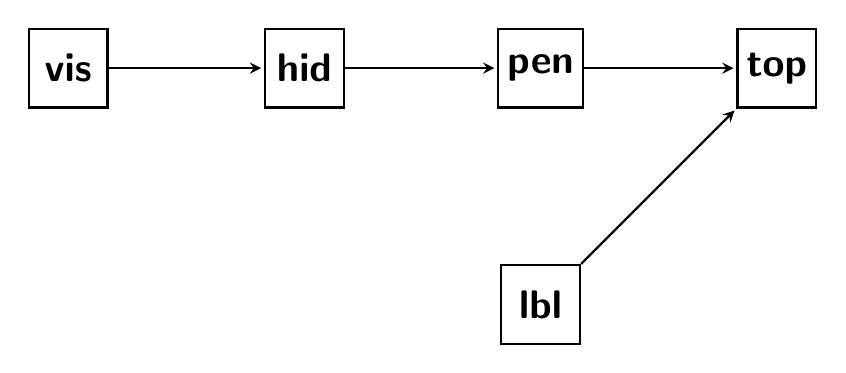
\begin{tikzpicture}[->,>=stealth,shorten >=1pt,auto,node distance=3cm,
                      thick,main node/.style={rectangle,draw,minimum size=1cm,font=\sffamily\Large\bfseries}]

    % Nodes
    \node[main node] (vis) {vis};
    \node[main node] (hid) [right of=vis] {hid};
    \node[main node] (pen) [right of=hid] {pen};
    \node[main node] (top) [right of=pen] {top};
    \node[main node] (lbl) [below of=pen] {lbl};

    % Paths
    \path[every node/.style={font=\sffamily\small}]
      (vis) edge node[below] {} (hid)
      (hid) edge node[below] {} (pen)
      (pen) edge node[below] {} (top)
      (lbl) edge node[right] {} (top);

  \end{tikzpicture}
  \caption{Illustration of the RBM stack with layers vis, hid, pen, top, and lbl.}
  \label{fig:rbm_stack}
\end{figure}
For this task, we pre-trained each layer or rather pre-trained the entire DBN according to the instructions and heavily inspired by the literature \cite{hinton2006fast} \cite{hinton2012practical}. Code was modified such that the output of a certain layer could be inputted to the next layer. Below are the results of the training and test dataset.

\begin{table}[ht]
\label{table: Results} % Optional: label for
\caption{Train and Test results on the dataset} % Optional: caption for the table
\centering % Center the table
\begin{tabular}{|c|c|} % Defines the columns; 'c' for centered, '|' for vertical lines

\hline % Horizontal line at the top of the table
Dataset & Results \\ % Table header
\hline % Horizontal line after the header
Training & 85.92\% \\ % First row
Testing & 86.10\% \\ % Second row
\hline % Horizontal line at the bottom of the table
\end{tabular}
\end{table}

Lastly, the DBN was used in generative mode. The function "generate" in the code template was modified to accommodate this and the generated figures were animated to see how well they generated figures. Below are the visualization of the weights on some of the images they drew.

\begin{figure}[htb]
    \centering
    \begin{subfigure}[b]{0.45\textwidth}
        \centering
        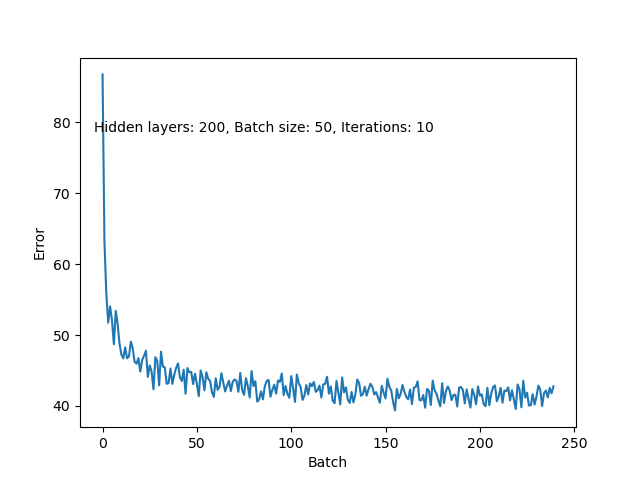
\includegraphics[width=\textwidth]{Labs/Lab 4/Rakin/plots/Hidden_layers_200_batch_50_iterations_10.png}
        \caption{No iterations}
        \label{fig:Lab4-iter1}
    \end{subfigure}
    %
    \begin{subfigure}[b]{0.45\textwidth}
        \centering
        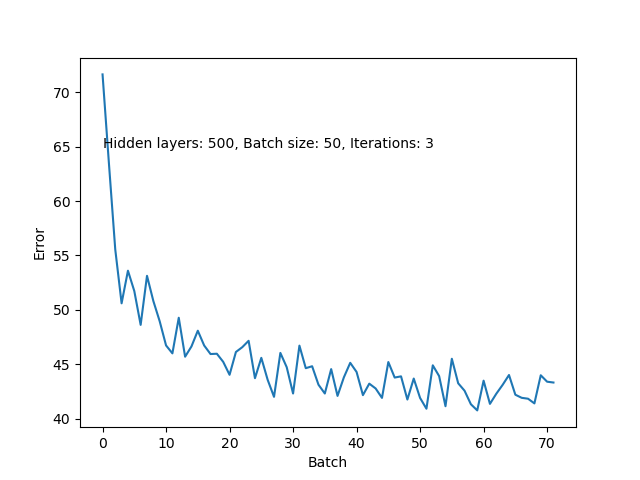
\includegraphics[width=\textwidth]{Labs/Lab 4/Rakin/plots/Hidden_layers_500_batch_50_iterations_3.png}
        \caption{First Iteration of Contrastive Divergence}
        \label{fig:Lab4-iter2}
    \end{subfigure}
    \caption{Comparison of None and First Iteration}
    \label{fig:Lab4-comparison-hiddenNodes}
\end{figure}



\section{Final remarks \normalsize{\textit{(max 0.5 page)}}}
\textit{Please share your final reflections on the lab, its content and your own learning. Which parts of the lab assignment did you find confusing or not necessarily helping in understanding important concepts and which parts you have found interesting and relevant to your learning experience? \\
Here you can also formulate your opinion, interpretation or speculation about some of the simulation outcomes. Please add any follow-up questions that you might have regarding the lab tasks and the results you have produced.}

\printbibliography


\end{document}
